\documentclass[tikz]{standalone}
\usetikzlibrary{math,calc}

\begin{document}
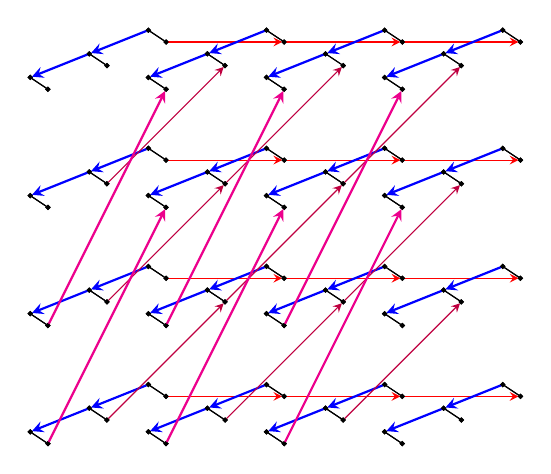
\begin{tikzpicture}[scale=1.5,
	every node/.style={draw,shape=circle,minimum size=.5mm,inner sep=0pt,outer sep=0pt,fill=black}, >=stealth]
	
	\tikzmath{
		integer \AMax, \BMax, \CMax;
		\AMax = 2;
		\BMax = 3;
		\CMax = 3;
	}
	
	\coordinate (x) at (-.5,-.2);
	\coordinate (y) at (1,0);
	\coordinate (z) at (0,1);
	\coordinate (w) at ($-.4*(y)-.5*(x)$);
	
	%---------------------------------------------
	
	\foreach \a in {0,...,\AMax} {
		\foreach \b in {0,...,\BMax} {
			\foreach \c in {0,...,\CMax} {
				\node (g\a_\b_\c_0) at ($\a*(x) + \b*(y) + \c*(z)$) {};
				\node (g\a_\b_\c_1) at ($\a*(x) + \b*(y) + \c*(z) + (w)$) {};
				\draw [] (g\a_\b_\c_0) --  (g\a_\b_\c_1); 
			}
		}
	}
	
	%---------------------------------------------%
	
	\tikzset{every path/.style={draw=red}}
	
	\draw [->] (g0_0_0_0) -- (g0_1_0_0);
	\draw [->] (g0_1_0_0) -- (g0_2_0_0);
	\draw [->] (g0_2_0_0) -- (g0_3_0_0);
	
	\draw [->] (g0_0_1_0) -- (g0_1_1_0);
	\draw [->] (g0_1_1_0) -- (g0_2_1_0);
	\draw [->] (g0_2_1_0) -- (g0_3_1_0);
	
	\draw [->] (g0_0_2_0) -- (g0_1_2_0);
	\draw [->] (g0_1_2_0) -- (g0_2_2_0);
	\draw [->] (g0_2_2_0) -- (g0_3_2_0);
	
	\draw [->] (g0_0_3_0) -- (g0_1_3_0);
	\draw [->] (g0_1_3_0) -- (g0_2_3_0);
	\draw [->] (g0_2_3_0) -- (g0_3_3_0);
	
	
	%---------------------------------------------%
	
	\tikzset{every path/.style={draw=blue,thick}}
	
	\foreach \b in {0,...,\BMax} {
		\foreach \c in {0,...,\CMax} {
			\draw [->] (g0_\b_\c_1) -- (g1_\b_\c_1);
			\draw [->] (g1_\b_\c_1) -- (g2_\b_\c_1);
		}
	}
	
	%---------------------------------------------%
	
	\tikzset{every path/.style={draw=purple}}
	
	\draw [->] (g1_0_0_0) -- (g1_1_1_0);
	\draw [->] (g1_1_0_0) -- (g1_2_1_0);
	\draw [->] (g1_2_0_0) -- (g1_3_1_0);
	
	\draw [->] (g1_0_1_0) -- (g1_1_2_0);
	\draw [->] (g1_1_1_0) -- (g1_2_2_0);
	\draw [->] (g1_2_1_0) -- (g1_3_2_0);
	
	\draw [->] (g1_0_2_0) -- (g1_1_3_0);
	\draw [->] (g1_1_2_0) -- (g1_2_3_0);
	\draw [->] (g1_2_2_0) -- (g1_3_3_0);
	
	%---------------------------------------------%
	
	\tikzset{every path/.style={}}
	
	\foreach \a in {0,...,\AMax} {
		\foreach \b in {0,...,\BMax} {
			\foreach \c in {0,...,\CMax} {
				\node (g\a_\b_\c_0) at ($\a*(x) + \b*(y) + \c*(z)$) {};
				\node (g\a_\b_\c_1) at ($\a*(x) + \b*(y) + \c*(z) + (w)$) {};
				\draw [] (g\a_\b_\c_0) --  (g\a_\b_\c_1); 
			}
		}
	}
	
	\tikzset{every path/.style={draw=magenta, thick}}
	
	\draw [->] (g2_0_0_0) -- (g2_1_2_0);
	\draw [->] (g2_1_0_0) -- (g2_2_2_0);
	\draw [->] (g2_2_0_0) -- (g2_3_2_0);
	
	\draw [->] (g2_0_1_0) -- (g2_1_3_0);
	\draw [->] (g2_1_1_0) -- (g2_2_3_0);
	\draw [->] (g2_2_1_0) -- (g2_3_3_0);
	
	%---------------------------------------------
	
\end{tikzpicture}
\end{document}